% Created 2020-08-01 Sat 17:06
% Intended LaTeX compiler: pdflatex
\documentclass[a4paper]{article}
\usepackage[utf8]{inputenc}
\usepackage[T1]{fontenc}
\usepackage{graphicx}
\usepackage{grffile}
\usepackage{longtable}
\usepackage{wrapfig}
\usepackage{rotating}
\usepackage[normalem]{ulem}
\usepackage{amsmath}
\usepackage{textcomp}
\usepackage{amssymb}
\usepackage{capt-of}
\usepackage{hyperref}
\usepackage[left=1in,top=1in,right=1in,bottom=1.5in]{geometry}
\usepackage{palatino}
\usepackage{sectsty}
\usepackage{engord}
\usepackage{cite}
\usepackage{graphicx}
\usepackage{setspace}
\usepackage[compact]{titlesec}
\usepackage[center]{caption}
\usepackage{multirow}
\usepackage{ifthen}
\usepackage{longtable}
\usepackage{color}
\usepackage{listings}
\usepackage{pdfpages}
\usepackage{nomencl}	% For glossary
\usepackage{pdflscape}	% For landscape pictures and environment
\usepackage{verbatim} 	% For multiline comment environments
\usepackage[table]{xcolor}
\usepackage{amssymb,amsmath}
\usepackage{fancyhdr} %For headers and footers
\pagestyle{fancy} %For headers and footers
\usepackage{lastpage} %For getting page x of y
\usepackage{float} %Allows the figures to be positioned and formatted nicely
\floatstyle{boxed} %using this
\restylefloat{figure} %and this command
\usepackage{url} %Formatting of yrls
\lhead{Paper example}
\chead{}
\rhead{\today}
\lfoot{Draft}
\cfoot{}
\rfoot{\thepage\ of \pageref{LastPage}}
\author{Bas Chatel}
\date{\today}
\title{Idea for Methodpaper example}
\hypersetup{
 pdfauthor={Bas Chatel},
 pdftitle={Idea for Methodpaper example},
 pdfkeywords={},
 pdfsubject={},
 pdfcreator={Emacs 26.3 (Org mode 9.3.7)}, 
 pdflang={English}}
\begin{document}

\maketitle

\section*{Introduction}
\label{sec:org4896f3c}
Here all modeling steps for turning qualitative knowledge into a quantitative system dynamics model are made concrete using a running example. We will first elaborate on the example problem statement, followed by the goals to be achieved. We will then describe the system, and finally, provide the hypotheses to be answered by modeling.

\subsection*{Problem}
\label{sec:orgbf646b5}
In this example, there is a group of four potato farmers noticing that their potato yield fluctuates significantly over the years. They have all invested in a greenhouse to have more control of the potato growing process. Using their greenhouses, however, they want to know more about the critical factors and how they can best control the environment to optimize potato yield.

\subsection*{Goal}
\label{sec:orgb987275}
The farmers want to apply systems thinking to understand more about the dynamics of potato population growth. It is in their best interest to:

\begin{enumerate}
\item Keep growth fluctuations low in order to have a steady income.
\item Know what are the best circumstances to grow potatoes in order to optimize yield.
\item Know what is the best timing to harvest.
\end{enumerate}

\subsection*{System}
\label{sec:orga2e61e4}
The farmers use greenhouses where they grow potato plants that need nutrients from the soil and a light source. In the greenhouses, they have full control over the light. The number of potato plants downregulates itself as they compete for space and light. Upon growing, the plants consume nutrients from the soil. Furthermore, the ground receives fertilization from a worm population that eats the leaves from, and therefore also drawn to the potato plants. However, when the soil is too rich in nutrients, the worm population will decrease as too high levels of nutrients are toxic to the worms. This system is depicted in figure \ref{fig:CLD} in the form of an aCLD.

\begin{figure}[t]
\centering
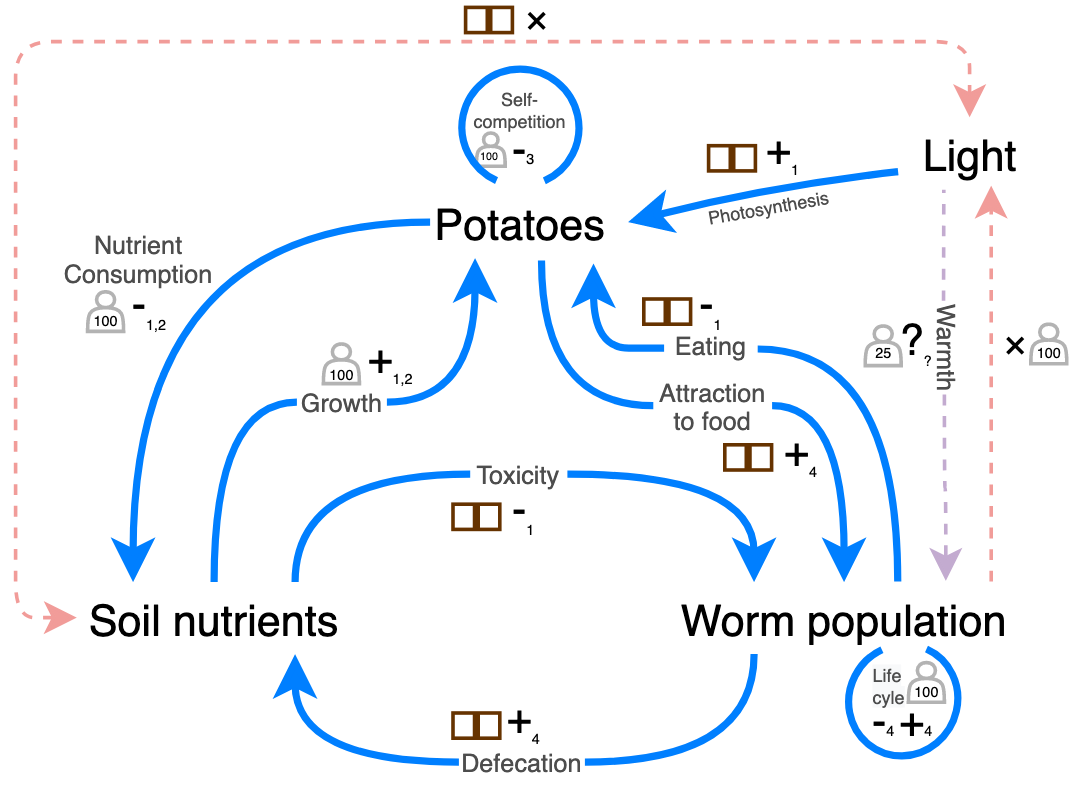
\includegraphics[width=0.75\linewidth]{network.png}
\caption{\label{fig:CLD}CLD of scenario}
\end{figure}

\subsection*{Hypothesis}
\label{sec:orgb8fa377}
The amount of light and the number of worms in the soil are the key factors to regulate to lead to a steady and optimized potato yield.

\clearpage
\subsection*{Data}
\label{sec:org1f7acb3}
The farmers decide to work together and agree to try and grow potatoes under similar conditions except for the strength of light. To keep things fair, they share the potato yield equally, so no single farmer has meager yield during the experiment. They tried to measure their potato population, the amount of nutrient richness of the soil, and the number of worms in the ground per square meter daily to provide us with data. This data is presented in figure \ref{fig:data} with some descriptive statistics in table \ref{tab:descr_data}.

\begin{figure}[h]
\centering
\includegraphics[width=1\linewidth]{data.png}
\caption{\label{fig:data}Data of four different greenhouses over 50 time-units. Measurements include strength of light, potato yield, amount of nutrients in the soil, and the number of worm.}
\end{figure}

\begin{table}[h]
\caption{\label{tab:descr_data}Descriptive statistics of data gathered by the farmers.}
\centering
\begin{tabular}{llrrrr}
 & Greenhouse & 1 & 2 & 3 & 4\\
\hline
Potatoes & Mean & 0.44 & 0.52 & 0.60 & 0.71\\
 & Std & 0.10 & 0.10 & 0.10 & 0.18\\
 & Min & 0.18 & 0.30 & 0.39 & 0.30\\
 & Max & 0.61 & 0.68 & 0.77 & 0.97\\
 & Missing & 60\% & 56\% & 58\% & 62\%\\
\hline
Nutrients & Mean & 0.54 & 0.45 & 0.53 & 0.48\\
 & Std & 0.10 & 0.09 & 0.09 & 0.06\\
 & Min & 0.38 & 0.26 & 0.39 & 0.39\\
 & Max & 0.77 & 0.68 & 0.74 & 0.71\\
 & Missing & 64\% & 54\% & 52\% & 52\%\\
\hline
Worms & Mean & 0.56 & 0.70 & 0.74 & 0.97\\
 & Std & 0.11 & 0.12 & 0.17 & 0.20\\
 & Min & 0.35 & 0.54 & 0.41 & 0.64\\
 & Max & 0.75 & 0.78 & 0.98 & 1.38\\
 & Missing & 58\% & 60\% & 52\% & 54\%\\
\hline
Lightstrength &  & 1.25 & 1.50 & 1.75 & 2.00\\
\end{tabular}
\end{table}

\clearpage
\subsection*{Labeling the causal loop diagram}
\label{sec:org61e712e}

\begin{figure}[h]
\centering
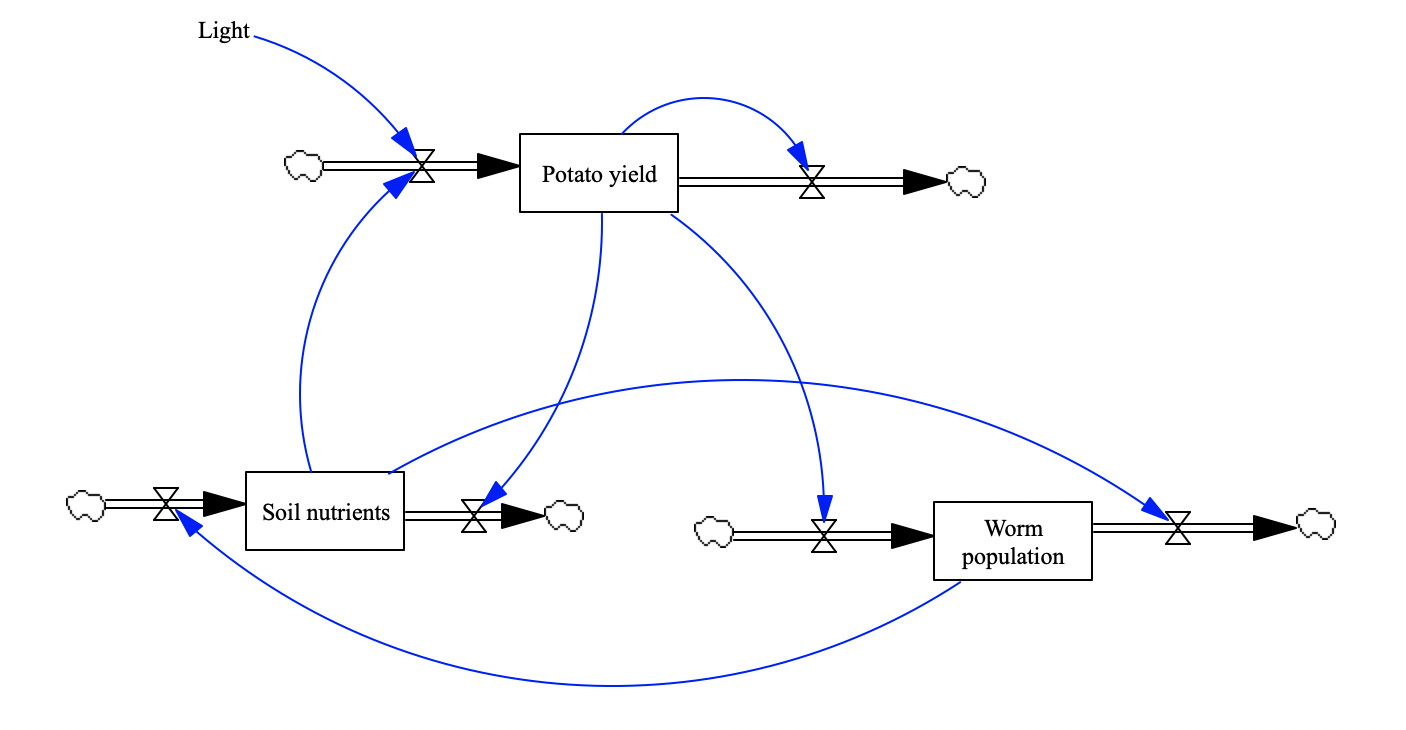
\includegraphics[width=1\linewidth]{image.png}
\caption{\label{fig:network}Network of scenario}
\end{figure}

\par\vspace{\baselineskip}\noindent

\par\vspace{\baselineskip}\noindent
\end{document}